% --------------------------------------------------------------------------
% Template for DCASE 2016 paper; to be used with:
%          dcase2016.sty  - DCASE 2016 LaTeX style file, and
%          IEEEbib.bst - IEEE bibliography style file.
% Adapted from spconf.sty and waspaa15.sty
% --------------------------------------------------------------------------

\documentclass{article}
\usepackage{dcase2016,amsmath,graphicx,url,times}
\usepackage{booktabs}
\usepackage{tikz}
\usepackage{amssymb}
\usetikzlibrary{arrows.meta}
%\usepackage{dcase2016,amssymb,amsmath,graphicx,times,url}

% Example definitions.
% --------------------
\def\defeqn{\stackrel{\triangle}{=}}
\newcommand{\symvec}[1]{{\mbox{\boldmath $#1$}}}
\newcommand{\symmat}[1]{{\mbox{\boldmath $#1$}}}

\newcommand{\la}{{\lambda}}
\newcommand{\lau}{{\lambda_1}}
\newcommand{\lad}{{\lambda_2}}

% Title.
% --------------------
\title{Binaural Scene Classification with Wavelet Scattering}

% Single addresses (uncomment and modify for single-address case).
% --------------------
%\name{Author(s) Name(s)\thanks{Thanks to XYZ agency for funding.}}
%\address{Author Affiliation(s)}
%
% For example:
% ------------
%\address{School\\
%       Department\\
%       Address}

% Two addresses
% --------------------
\twoauthors
  {Vincent Lostanlen\sthanks{This work is supported by the ERC InvariantClass grant 320959. The source code to reproduce figures and experiments is freely available at \protect\url{http://www.github.com/lostanlen/dcase2016}.}}
    {D\'{e}partement d'Informatique \\ \'{E}cole normale sup\'{e}rieure \\ Paris, France \\
     vincent.lostanlen@ens.fr}
  {Joakim And\'{e}n\footnotemark[1]}
    {Program in Applied and Computational Mathematics \\ Princeton University \\
     Princeton, NJ, USA \\
     janden@math.princeton.edu}

\begin{document}

\ninept
\maketitle

\begin{sloppy}

\begin{abstract}
This technical report describes our contribution to the scene classification task of the 2016 edition of the IEEE AASP Challenge for Detection and Classification of Acoustic Scenes and Events (DCASE). Our computational pipeline consists of a gammatone scattering transform, logarithmically compressed and coupled with a per-frame linear support vector machine. At test time, frame-level labels are aggregated over the whole recording by majority vote. During the training phase, we propose a novel data augmentation technique, where left and right channels are mixed at different proportions to introduce invariance to sound direction in the training data.
\end{abstract}

\begin{keywords}
scattering transform, wavelets, auditory scene classification, orientation invariance, support vector machine
\end{keywords}

\section{System Outline}
\label{sec:outline}
The system used for the scene classification task is illustrated in Figure \ref{fig:outline}. Each recording is decomposed using a time scattering transform, which provides a signal representation that is locally invariant to time-shifting and stable to time-warping deformation. Since small changes in timing have little relevance to the auditory scene of a particular recording, this invariance reduces the variability of the data without necessarily hampering discriminability. The averaging scale of the scattering transform is fixed to be $740~\mathrm{ms}$. In order to account for the varying orders of magnitude across frequencies, we then apply a logarithmic compression to the data. Each recording is thus represented as a sequence of logarithmically compressed scattering vectors.

Due to the stereophonic nature of the recordings, we augment the training data by constructing monophonic signals with different mixing proportions, effectively providing invariance to sound direction. At the training stage, a linear support vector machine (SVM) classifier is trained using the sequences obtained from the training data. For each recording in the testing set, the classifier is applied to all scattering vectors in the recording, yielding a class for each vector. The class of the entire recording is then determined by majority vote. Evaluating this system on the standard four train-test splits in the development data, we obtain an average accuracy of $79.4\%$.

\begin{figure}
\begin{center}
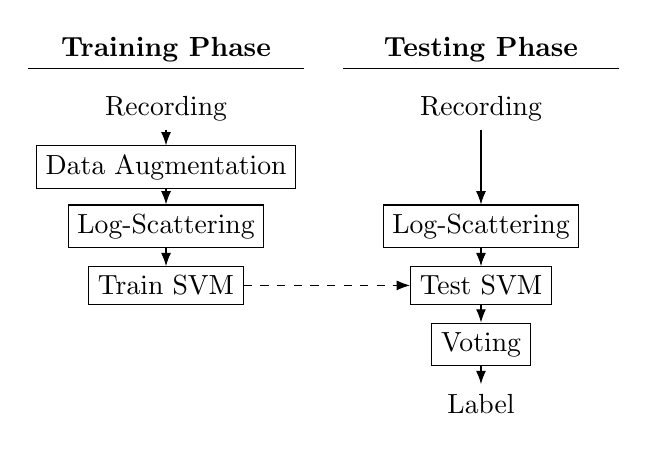
\begin{tikzpicture}
\node (train heading) at (2, 6) {\textbf{Training Phase}};
\draw (0.25, 5.75) -- (3.75, 5.75);
\node (train data) at (2, 5.25) {Recording};
\node[draw,rectangle] (train augment) at (2, 4.50) {Data Augmentation};
\node[draw,rectangle] (train scatt) at (2, 3.75) {Log-Scattering};
\node[draw,rectangle] (train svm) at (2, 3) {Train SVM};
\draw[-{Latex}] (train data) -- (train augment);
\draw[-{Latex}] (train augment) -- (train scatt);
\draw[-{Latex}] (train scatt) -- (train svm);

\node (test heading) at (6, 6) {\textbf{Testing Phase}};
\draw (4.25, 5.75) -- (7.75, 5.75);
\node (test data) at (6, 5.25) {Recording};
\node[draw,rectangle] (test scatt) at (6, 3.75) {Log-Scattering};
\node[draw,rectangle] (test svm) at (6, 3) {Test SVM};
\node[draw,rectangle] (test vote) at (6, 2.25) {Voting};
\node (test label) at (6, 1.5) {Label};
\draw[-{Latex}] (test data) -- (test scatt);
\draw[-{Latex}] (test scatt) -- (test svm);
\draw[-{Latex}] (test svm) -- (test vote);
\draw[-{Latex}] (test vote) -- (test label);

\draw[dashed,-{Latex}] (train svm) -- (test svm);
\end{tikzpicture}
\end{center}
\caption{
\label{fig:outline}
The scattering classification system proposed for the scene classification challenge. During the training phase, the data is augmented by mixing the left and right channels at various proportions. The log-scattering vectors are then computed and used to train a linear SVM. This SVM is then used to classify the sequence of log-scattering vectors for each test recording. The resulting sequence of labels is reduced to a single recording label through majority vote.
}
\end{figure}


\section{Scattering Representation}
\label{sec:scattering}

The scattering transform was introduced by S. Mallat as a signal representation that is invariant to translations and stable to deformation \cite{stephane}. It has had success in classifying images \cite{joan}, audio \cite{dss}, and biomedical signals \cite{embs}. For audio signals, translation corresponds to time-shifting, while deforming a signal warps it in time. Both of these transformations have little to no effect on the semantic content of an audio signal, so reducing their influence enables us to train more accurate classifiers using limited training data. A brief review of the scattering transform is provided in this section.

\begin{figure}
\begin{center}
\begin{tikzpicture}
\useasboundingbox[red] (-0.25, -0.5) rectangle (8.25, 2);
\node (omlabel1) at (3.5, 1) {$\omega$};
\draw[-{Latex[length=2mm]}] (0, 1) -- (omlabel1);
\draw[-{Latex[length=2mm]}] (0, 1) -- (0, 2);
\node[anchor=south west,inner sep=0] at (0, 0) {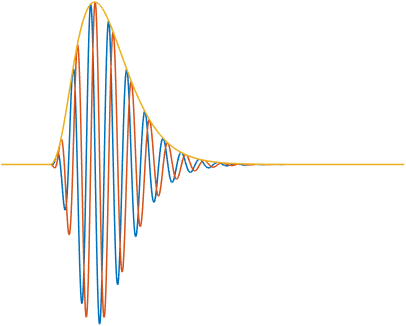
\includegraphics[height=2cm,width=3cm]{gammatone_Q4.png}};
\node at (2, -0.25) {(a)};

\node (omlabel2) at (8, 1) {$\omega$};
\draw[-{Latex[length=2mm]}] (4.5, 1) -- (omlabel2);
\draw[-{Latex[length=2mm]}] (4.5, 1) -- (4.5, 2);
\node[anchor=south west,inner sep=0] at (4.5, 0) {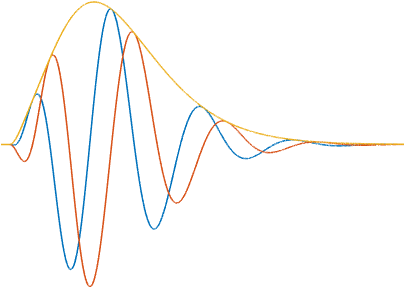
\includegraphics[height=2cm,width=3cm]{gammatone_Q1.png}};
\node at (6.5, -0.25) {(b)};
\end{tikzpicture}
\caption{
\label{fig:gammatones}
Fourier transforms $\widehat{\psi}(\omega)$ of Gammatone mother wavelets with quality factors (a) $Q = 4$ and (b) $Q = 1$. Blue and red oscillations represent the real and imaginary parts. The orange envelope represents the complex modulus. Note that the Fourier transforms are zero in the negative frequencies.}
\end{center}
\end{figure}

First, for a signal $x$, let us define its Fourier transform $\widehat{x}$ by
\begin{equation}
	\widehat{x}(\omega) = \int_{\mathbb{R}} x(u) e^{-i\omega u}\,du.
\end{equation}
Given an analytic filter $\psi$ with Fourier transform $\widehat{\psi}$ concentrated around the dimensionless frequency $1$, we define a wavelet filter bank $\{\psi_\lambda\}_{\lambda>0}$ by dilating $\psi$, called the mother wavelet, to obtain
\begin{equation}
	\psi_\lambda(t) = \lambda \psi(\lambda t).
\end{equation}
The analyticity of $\psi$ forces its Fourier transform to be zero for negative frequencies. The wavelet filters $\psi_\lambda$ are also analytic and since $\widehat{\psi}$ is centered around frequency $1$, $\widehat{\psi}_\la$ is centered around $\lambda$.

A function $\psi$ that fulfills our conditions is the pseudo-analytic Gammatone wavelet, illustrated in Figure \ref{fig:gammatones}. Its form is given explicitly by
\begin{equation}
	\psi(t) = \left((n-1)t^{n-2}+ i t^{n-1}\right)e^{-(b + i) t}\, 1_{[0,\infty)}(t),
\end{equation}
where the bandwidth parameter $b$ is roughly proportional to $2^{-1/Q}$ and $Q$ is the desired quality factor, i.e. the ratio of the center frequency to the half-maximum bandwidth in the Fourier domain. To begin with, we shall take $Q = 4$.

Given a signal $x$, we decompose it using the wavelet filter bank to obtain
\begin{equation}
	x \ast \psi_\lau(t) \quad \mathrm{for~}\lau>0,
\end{equation}
known as the wavelet decomposition of $x$. We have denoted the standard convolution operator by $\ast$. The dilation structure of the wavelet filter bank means that we do not need to sample $\lau$ continuously. Rather, it is sufficient to sample $\lau$ as $2^{j/Q}$, where $Q$ is the quality factor of the mother wavelet $\psi$. This means that we sample uniformly in log-frequency $\log \lau$.

The wavelet decomposition itself is very sensitive to time-shifting and time-warping, which can be partially mitigated by taking the complex modulus. The result is known as the wavelet scalogram and we denote it by
\begin{equation}
	x_1(t, \log \lau) = | x \ast \psi_\lau(t) |.
\end{equation}

The scalogram provides a useful representation of the time-frequency content of a signal. At a given point $(t, \log \lau)$, it gives the intensity of $x$ at time $t$ and log-frequency $\log \lau_1$. However, it does not have the desired invariance and stability properties. To achieve this, we average the scalogram in time using a lowpass filter $\phi_T(t)$ of duration $T$ to give
\begin{align}
	\nonumber
	S_1 x(t, \log \lau) &= x_1(\cdot, \log \lau) \ast \phi_T(t) \\
	&= | x \ast \psi_\lau | \ast \phi_T(t).
\end{align}
In our configuration $\phi_T$ is given by a Gabor filter centered at frequency $0$ with the desired bandwidth $T$ in time. The coefficients $S_1 x$ are known as first-order time scattering coefficients and are comparable to the commonly used mel-frequency spectrogram coefficients \cite{davis-mermelstein}.

The averaging by $\phi_T$ discards fine-scale temporal structure in the scalogram $x_1$. To recover this, we calculate a second wavelet decomposition on the scalogram along the time axis. Instead of the quality factor $Q = 4$ used in the first decomposition, we now use $Q = 1$. As before, we compute the complex modulus and obtain
\begin{align}
	\nonumber
	x_2(t, \log \lau, \log \lad) &= x_1(\cdot, \log \lau) \ast \psi_\lad(t) \\
	&= |\,| x \ast \psi_\lau | \ast \psi_\lad (t) |.
\end{align}
This second-order wavelet scalogram describes the modulation structure of the frequency band centered at $\log \lau$ of the first-order scalogram $x_1$. It is therefore closely related to modulation spectrograms \cite{atlas,hermansky}, but are defined using wavelet decompositions instead of short-time Fourier transforms.

Again, to obtain invariance, the second-order scalogram $x_2$ is averaged in time using the lowpass filter $\phi_T$ to give
\begin{align}
	\nonumber
	S_2 x(t, \log \lau, \log \lad) &= x_2(\cdot, \log \lau, \log \lad) \ast \phi_T(t) \\
	&= |\,| x \ast \psi_\lau | \ast \psi_\lad | \ast \phi_T(t),
\end{align}
which are known as second-order time scattering coefficients. Like modulation spectrograms, these coefficients provide information on the modulation structure of the signal $x$ at log-frequency $\log \lau$, but do so in a stable manner due to the wavelet construction. In this way, they are more closely related to constant-Q averaged modulation spectrograms \cite{ellis-mcdermott,thompson2003non}. We note that the above procedure can be continued for third- and higher-order scattering coefficients, but that for most applications, first- and second-order coefficients suffice.

Concatenating all the first-order scattering coefficients into one vector
\begin{equation}
	S_1x(t) = \{S_1x(t, \log \lau)\}_{\lau>0},
\end{equation}
and doing the same for the second-order coefficients
\begin{equation}
	S_2x(t) = \{S_2x(t, \log \lau, \log \lad\}_{\lau>0, \lad>0},
\end{equation}
we can combine all of them into one scattering vector at time $t$
\begin{equation}
	Sx(t) = \{S_1x(t), S_2x(t)\}.
\end{equation}

It is important here to remark that, although the above formulas cover continuous domains in $t$, $\log \lau$, and $\log \lad$, these variables can all be sampled discretely without great loss of information. As mentioned earlier, $\log \lau$ and $\log \lad$ can be sampled uniformly with a step proportional to $1/Q$. In addition, the lowpass nature of the scalogram $x_1$ in time ensures that many coefficients in $x_2$ will be negligible for large values of $\log \lad$. As a result, these can be safely excluded from the transform. Finally, the lowpass filtering by $\phi_T$ ensures that we can sample the final scattering vector $Sx$ along multiples of $T/4$ in time.

\section{Scattering Post-Processing}
\label{sec:post}

Instead of feeding the raw scattering vectors into the SVM classifier, we process them to facilitate model building by reducing their dynamic range and standardizing their variability. Specifically, we first compute the log-scattering coefficients by taking the logarithm of each value in the scattering vector to get
\begin{equation}
	\log S_1 x(t, \log \lau) = \log \left( | x \ast \psi_\lau | \ast \phi_T(t) \right)
\end{equation}
in the first order and
\begin{equation}
	\log S_2 x(t, \log \lau, \log \lad) = \log \left( |\,| x \ast \psi_\lau | \ast \psi_\lad | \ast \phi_T(t) \right)
\end{equation}
in the second order. These are combined across all log-frequencies $\log \lau$ and $\log \lad$ as before to yield a log-scattering vector $\log Sx(t)$.

The log-scattering coefficients are better suited for audio classification since audio amplitudes can vary across several orders of magnitude without significantly changing the content of the signal. This is often characterized as the Weber-Fechner law in psychoacoustics.

In addition, we diagonally standardize the coefficients to have mean zero and unit variance. To do this for our train-test splits, we calculate the mean and variance for each scattering coefficient across our training data and then use this to standardize both the training and testing data for the current split. This helps improve the conditioning of the SVM training since all values are in the same numerical range.

\section{Data Augmentation}
\label{sec:augment}

Most acoustic scene datasets are recorded according to a binaural protocol, i.e. with a pair of in-ear microphones \cite{Wang2006}. This protocol provides a realistic description of the spatial auditory environment, as it reproduces the natural listening conditions of humans. In particular, the interaural level difference (ILD) between the left and right channels depends on the direction of each sound source that make up the scene with respect to the listener \cite{Blauert2004}. Yet, since the microphone location and direction vary across instances of the same class, the signal representation should be invariant to these parameters.

In order to achieve invariance to changes in direction, averaging the left and right channels into a monophonic signal is by far the most widespread approach.  If these are denoted by $x_{\mathsf{L}}$ and $x_{\mathsf{R}}$, respectively, we would thus have
\begin{equation}
	x_{\mathsf{M}}(t) = \frac{1}{2} x_{\mathsf{L}}(t) + \frac{1}{2} x_{\mathsf{R}}(t),
\end{equation}
where $x_{\mathsf{M}}$ is the mixed signal. However, it favors the center of the scene while attenuating lateral cues. Indeed, if $x_{\mathsf{L}}$ is zero and $x_{\mathsf{R}}$ contains the entire signal, the resulting mixed signal $x_{\mathsf{M}}$ will have a lower amplitude.

To create the desired invariance without overemphasizing the central direction, we calculate multiple combinations of the left and right channels into the monophonic signal $x_{\alpha}$ using the formula
\begin{equation}
x_{\alpha}(t) =
\dfrac{1+\alpha}{2} x_{\mathsf{L}}(t) +
\dfrac{1-\alpha}{2} x_{\mathsf{R}}(t),
\end{equation}
where $\alpha$ determines the mixing between the channels. Note that taking $\alpha = 0$ gives us the center mixed signal $x_{\mathsf{M}}$ described above.

In following experiments, we set $\alpha$ to $-1$, $\frac{1}{2}$, $0$, $+\frac{1}{2}$, and $+1$. This is a form of data augmentation since $5$ monophonic signals are obtained from each binaural recording in the training set, increasing its size. At test time, only the center combination ($\alpha = 0$) is used to classify the recording.

\section{Classifier}
\label{sec:classifier}

Given the recordings in a training set, we compute their scattering vectors as described in Section \ref{sec:scattering}. Each recording being $30~\mathrm{s}$ long and the averaging window set at $T = 740~\mathrm{ms}$, this results in $160$ scattering vectors per recording, since $Sx$ is sampled at intervals of size $T/4 = 186~\mathrm{ms}$. From these, log-scattering vectors $\log Sx$ are computed as outlined in Section \ref{sec:post} and their mean and variance are computed across all recordings in the training set. These values are then used to standardize the log-scattering vectors to have mean zero and unit variance.

These log-scattering vectors are then fed, along with the class label of the recording they are extracted from, into the training algorithm for a linear SVM. An SVM is a binary linear classifier which is trained by finding the hyperplane that best separates two classes while minimizing training error \cite{vapnik}. In our system, we used the LIBLINEAR library \cite{liblinear}. Since the SVM is formulated as a binary classifier, a one-versus-all scheme is used to generalize its results to a multi-class setting.

To train the SVM, a cost parameter $C$ is used to determine the trade-off between penalizing errors on the training data and the maximization of discriminatory margin. In our case, we saw very little difference in performance when varying this parameter, which suggests that there is little conflict between these two objectives and that the data is therefore close to linearly separable. As a result, we set $C$ equal to $1$.

Once the SVM is trained, we feed it log-scattering vectors from the testing set. As discussed in Section \ref{sec:post}, these are first standardized by the mean and variance derived from the training set. Again, a $30~\mathrm{s}$-recording in the testing set yields $160$ log-scattering vectors, which means that the SVM returns $160$ different class labels for a single recording. To obtain a label for the entire recording, we perform a majority vote among all the labels corresponding to the individual log-scattering vectors. This type of approach to aggregating representation vectors along a time series is known as a late integration scheme \cite{kittler}.

\section{Numerical Results}
\label{sec:results}

\begin{table}[t]
\begin{center}
\begin{tabular}{lcc}
\toprule
Scene & Baseline & Temporal scattering \\
\midrule
beach & $74.6 \pm 18.9$ & $83.5 \pm \phantom{0}7.1$ \\
bus & $58.2 \pm 18.3$ & $88.8 \pm 11.4$ \\
cafe/restaurant & $85.1 \pm 10.8$ & $64.5 \pm \phantom{0}8.3$ \\
car & $69.1 \pm 20.8$ & $94.9 \pm \phantom{0}6.1$ \\
city\_center & $89.6 \pm \phantom{0}9.2$ & $91.7 \pm \phantom{0}9.4$ \\
forest\_path & $72.4 \pm 23.8$ & $93.8 \pm \phantom{0}7.8$ \\
grocery\_store & $74.1 \pm 13.7$ & $90.9 \pm \phantom{0}6.9$ \\
home & $78.1 \pm 17.7$ & $56.2 \pm 23.9$ \\
library & $65.1 \pm 23.3$ & $82.0 \pm 13.0$ \\
metro\_station & $85.2 \pm 15.6$ & $96.0 \pm \phantom{0}2.3$ \\
office & $90.8 \pm 16.0$ & $87.5 \pm 21.7$ \\
park & $25.6 \pm 11.0$ & $75.4 \pm \phantom{0}7.4$ \\
residential\_area & $75.1 \pm 19.4$ & $44.2 \pm 15.0$ \\
train & $34.1 \pm \phantom{0}7.2$ & $58.3 \pm 10.0$ \\
tram & $85.4 \pm 13.9$ & $83.7 \pm 12.2$ \\
\bottomrule
Average & $70.8 \pm \phantom{0}2.6$ & $79.4 \pm \phantom{0}3.0$ \\
\end{tabular}

\end{center}
\caption{\label{table:development-results} Classification results obtained through cross-validation on the development data for the DCASE 2016 scene classification challenge. The mean and standard deviation of the percentage correct in each class is provided along with the average across classes.}
\end{table}

To evaluate the time scattering system proposed above, we apply it to the development data provided with the DCASE 2016 scene classification challenge. This dataset is divided into four folds, which can be used to form train-test splits by training on three folds and testing on the remaining fold. This cross-validation procedure provides an estimate of the mean classification accuracy along with its variability due to differing training sets.

The results for the entire system is provided in Table \ref{table:development-results}. It is to be noted that while performance is quite good for most classes, certain classes (``cafe/restaurant'', ``residential\_area'', and ``train'') perform very poorly. These scenes are relatively quiet, with few characteristic sounds present, which could explain the difficulty in classifying them well. The exact cause for this difference in performance merits further study.

Despite these problems, the system provides a significant improvement over the baseline system, which consists of mel-frequency cepstral coefficients (MFCCs) modeled using Gaussian mixture models (GMMs) \cite{heittola}. Since the scattering representation takes into account the modulation structure of the scalogram in addition to the average spectral envelope captured by MFCCs, this improvement in performance is to be expected. We expect that further increases in performance can be achieved for this task by introducing more sophisticated extensions of the scattering transform such as the joint time-frequency scattering transform \cite{joint}.

\bibliographystyle{IEEEtran}
\bibliography{Lostanlen_dcase2016}

\end{sloppy}

\end{document}


